\documentclass[12pt,xcolor=dvipsnames]{article}
\usepackage[utf8]{inputenc}
\usepackage[vietnamese]{babel}
\usepackage{amstext,latexsym,amsbsy,amssymb,amsmath,amsthm,amsfonts,exscale,eucal}
\usepackage{appendix}
\usepackage{algorithm}
\usepackage{graphicx}
\usepackage{xcolor}
\usepackage{hyperref}
\usepackage{indentfirst}
\usepackage{enumitem}
\usepackage{diagbox}
\usepackage{booktabs}

\usepackage[left=2.00cm, right=2.00cm, top=2.00cm, bottom=2.00cm]{geometry}
\setlength{\parskip}{5pt}%khoảng cách dòng
\renewcommand{\baselinestretch}{1.15}
\theoremstyle{definition}
\newtheorem{vd}{Ví dụ}[section]
\newtheorem*{giai}{Giải}
\newtheorem{bt}{Bài tập}
\renewcommand{\l}{\left}
\renewcommand{\r}{\right}
\date{}

\begin{document}
\begin{bt}
(Bootstrap aggregating - Bagging). Xét dữ liệu \texttt{breast\_cancer.csv}.
\begin{enumerate}
    \item[(a)] Chia dữ liệu 70-30. Huấn luyện cây phân loại. Đánh giá Accuracy/AUC. Nhận xét về độ ổn định.
    \item[(b)] Bagging thủ công ($B=200$). Tính Accuracy/AUC.
    \item[(c)] Lặp lại train/test 50 lần. Tính phương sai Accuracy. So sánh Bagging vs Cây đơn lẻ.
    \item[(d)] So sánh với Random Forest ($ntree=200$). Giải thích.
\end{enumerate}
\end{bt}

\begin{giai}
\textbf{1. Cây phân loại đơn lẻ (Decision Tree)}

Kết quả chạy thử nghiệm với hai random seed khác nhau:
\begin{itemize}
    \item Seed 123: Accuracy = 0.9123, AUC = 0.9574
    \item Seed 456: Accuracy = 0.8947, AUC = 0.9304
\end{itemize}
\textit{Nhận xét:} Kết quả của cây quyết định thay đổi đáng kể khi thay đổi seed (cách chia dữ liệu). Điều này cho thấy cây quyết định là một mô hình có phương sai cao (high variance), tức là rất nhạy cảm với dữ liệu huấn luyện.

\textbf{2. Bagging (Bootstrap Aggregating)}

Thực hiện Bagging với $B=200$ cây con, kết hợp dự đoán bằng trung bình xác suất:
\begin{itemize}
    \item Accuracy: 0.9415
    \item AUC: 0.9904
\end{itemize}
Mô hình Bagging cải thiện đáng kể cả độ chính xác và chỉ số AUC so với cây đơn lẻ.

\textbf{3. Giảm phương sai (Variance Reduction)}

Lặp lại quy trình train/test 50 lần để ước lượng phân phối của độ chính xác:

\begin{table}[h]
\centering
\begin{tabular}{lcc}
\toprule
\textbf{Mô hình} & \textbf{Accuracy Trung bình} & \textbf{Phương sai (Variance)} \\
\midrule
Single Decision Tree & 0.9265 & 0.000458 \\
Bagging ($B=200$) & 0.9443 & 0.000373 \\
Random Forest & 0.9594 & 0.000197 \\
\bottomrule
\end{tabular}
\caption{So sánh hiệu năng qua 50 lần lặp}
\end{table}

Phần trăm giảm phương sai của Bagging so với Cây đơn lẻ:
\[
\text{Reduction} = \frac{\text{Var}_{\text{Tree}} - \text{Var}_{\text{Bagging}}}{\text{Var}_{\text{Tree}}} \approx \frac{0.000458 - 0.000373}{0.000458} \approx 18.56\%
\]
Bagging giúp giảm phương sai bằng cách lấy trung bình của nhiều mô hình nhiễu (noisy models), giúp đường biên phân chia mượt mà và ổn định hơn.

\begin{center}
    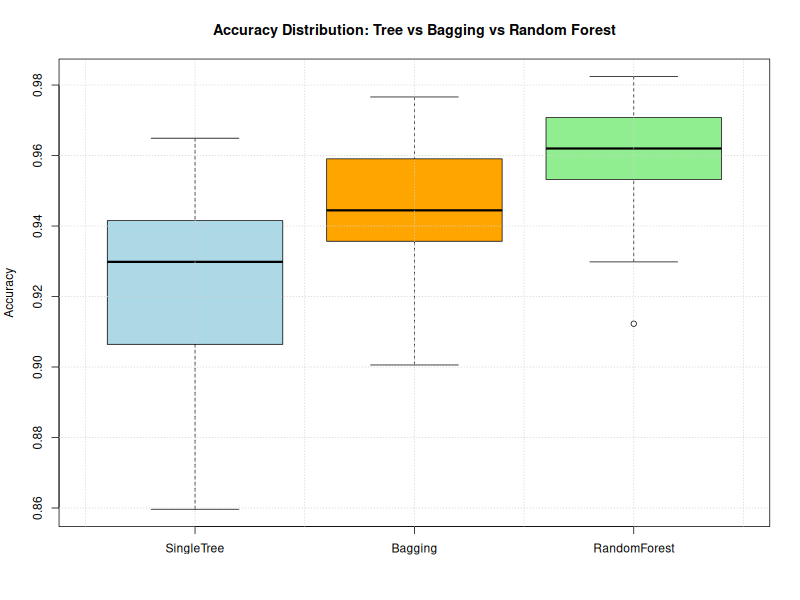
\includegraphics[width=0.8\textwidth]{bagging_variance_comparison.png}
\end{center}

\textbf{4. So sánh với Random Forest}

Random Forest đạt độ chính xác cao nhất (0.9594) và phương sai thấp nhất (0.000197). 

\textit{Giải thích:}
\begin{itemize}
    \item \textbf{Bagging:} Các cây con trong Bagging vẫn có tương quan cao (correlated) với nhau vì chúng đều có xu hướng chọn các biến quan trọng nhất (ví dụ: kích thước khối u) để phân nhánh ở các nốt đầu tiên.
    \item \textbf{Random Forest:} Tại mỗi nốt phân chia, thuật toán chỉ xem xét một tập con ngẫu nhiên các biến (\textit{random feature selection}). Điều này buộc các cây phải sử dụng các biến khác nhau, làm giảm sự tương quan giữa các cây (de-correlation).
    \item Khi các cây ít tương quan hơn, việc lấy trung bình sẽ giảm phương sai hiệu quả hơn theo công thức: $\text{Var}(\bar{X}) = \rho \sigma^2 + \frac{1-\rho}{B}\sigma^2$. Random Forest giảm $\rho$, do đó giảm tổng phương sai tốt hơn Bagging thuần túy.
\end{itemize}

\textbf{Mã nguồn:} File \texttt{exercise\_04.R} chứa toàn bộ code thực hiện mô phỏng.
\end{giai}
\end{document}
